\chapter{Methodology}

This chapter will provide a comprehensive solution to the problem statement along with the math required to prove its correctness and to help implement it.\newline

Input: A stream of monocular Images in perspective view with a moving person/object.\newline

Output: A trajectory of the person/object moving through the image space.\newline

Idea: The idea is to first find the walls, the roof, and the floor of the confined space/room. Then, using these walls, figure out the perspective view that the image exists in and overlay some points on the image as a reference for the coordinate system. Once we have the coordinate system in place, we can start detecting the subject using a neural network. Post detection, we convert the location of the subject from 2-dimensional image space to the 3-dimensional coordinate system by the usage of angular ratios calculated by the extension of projection lines from one of the vanishing points. Continual calculation of these 3-D locations yields a trajectory. Further, to make the detection more efficient, we start predicting zones in the image space where the subject might be present in the next frame, and the detection algorithm only looks for the object/person in the predicted zone until the object/person can’t be found or detected in the predicted zone anymore. If the subject is covered by another object, then the focus shifts to the object covering our subject, and we wait for our subject to re-emerge. If the subject does not resurface, the focus shifts back to the entire frame.\newline

We will divide the problem into three subproblems: 1) Mapping the room, 2) Calculating the coordinates of the person/object in consideration, and 3) Following the person/object as he moves through the image space essentially tracking him.\newline

\section{Mapping the room}

To effectively implement the coordinate calculating method proposed further in this chapter, we need to find the vanishing points effectively, and to do so we need to detect the walls and the corners present in the room. Using the edges of the walls to mark the lines on them and extending these lines further, we can calculate the vanishing points. This can be done in a few ways. The first is to use edge detection filters to find all the edges present in the space lines over these edges and extend these lines to find three line-intersection points, which represent the corners of the room. Using a combination of the lines and the corners to find multiple line intersection points will lead us to the vanishing points. This, however, is a slow and computationally expensive method, and can easily be led in the wrong direction by the presence of other objects in the room, that are not perfectly angular, such as a ball or a chair with a curved back. Another way to do so would be to use image segmentation. Once the wall boundaries are found, we can use a line-detection algorithm to extend the boundaries of the segmented areas and find multiple line-intersection points that represent potential vanishing points. Because segmenting to the ground truth is not easy, there are always errors that occur in the method while finding the exact position of the vanishing point is hard. However, our method helps us to get an area of the image that has a high probability of containing the weighted vanishing point. We can find the centroid of the area that we obtain from the algorithm and use that as the weighted vanishing point. The weighted vanishing point would represent the centroid of all the vanishing points present in the image, depending upon the perspective view of the image.

\section{Calculating The Coordinates}


\begin{figure}[H]
    \centering
    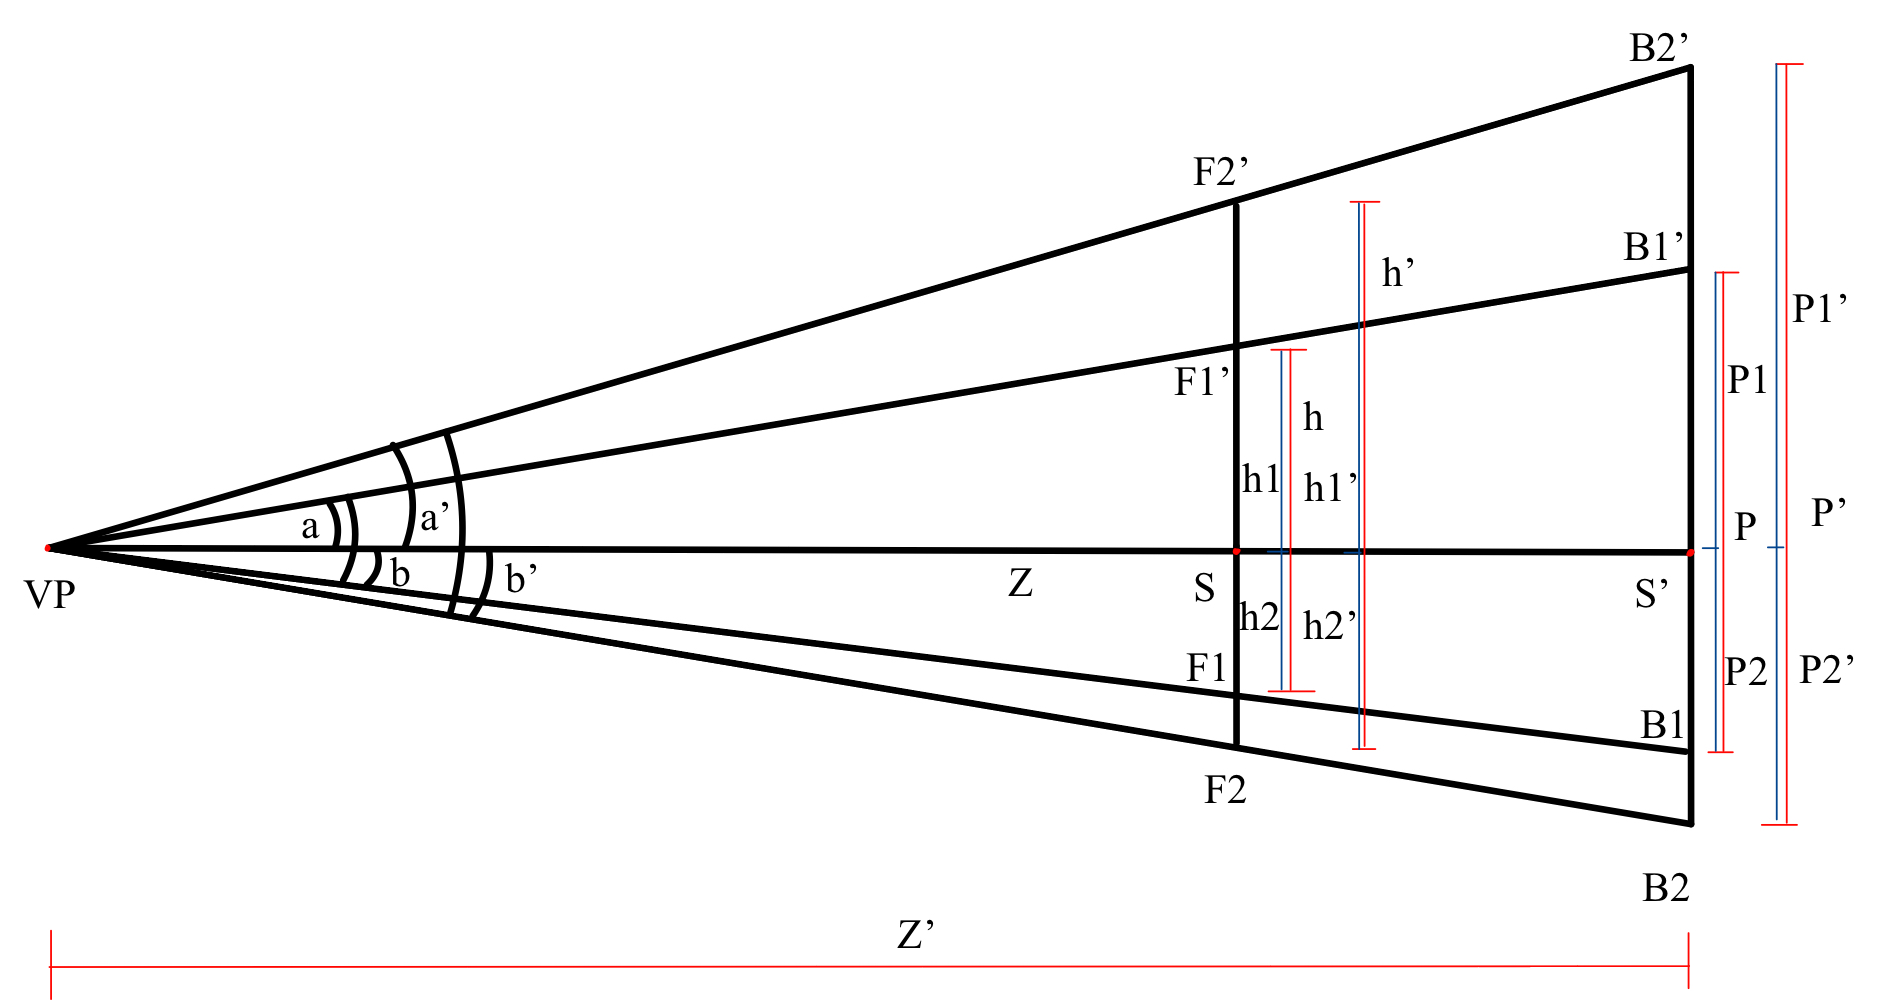
\includegraphics[width=1.0\textwidth]{Calculations1.jpeg}
    \caption{Projections from vanishing point}
    \label{fig: Projections from vanishing point}
\end{figure}

    \begin{Equation}[H]
        \begin{equation}
            \label{equation1}
            \tan(a) + \tan(b) = \frac{h_1}{Z} + \frac{h_2}{Z} = \frac{h}{Z}
        \end{equation}
        \caption{equation$1$}
    \end{Equation}
    
    \begin{Equation}[H]
        \begin{equation}
        \label{eq:equation1}
            \tan(a) + \tan(b) = \frac{P_1}{Z} + \frac{P_2}{Z} = \frac{P}{{Z'}}
        \end{equation}
        \caption{equation$2$}
    \end{Equation}
    
    \begin{Equation}[H]
        \begin{equation}
        \label{eq:equation1}
            \frac{Z}{Z'} = \frac{h}{P}
        \end{equation}
        \caption{equation$3$}
    \end{Equation}
    
    \begin{Equation}[H]
        \begin{equation}
        \label{eq:equation1}
            \tan(a') + \tan(b') = \frac{{h_1'}}{Z} + \frac{{h_2'}}{Z} = \frac{{h'}}{Z}
        \end{equation}
        \caption{equation$4$}
    \end{Equation}
    
    \begin{Equation}[H]
        \begin{equation}
        \label{eq:equation1}
            \tan(a') + \tan(b') = \frac{{P_1'}}{Z} + \frac{{P_2'}}{Z} = \frac{{P'}}{{Z'}}
        \end{equation}
        \caption{equation$5$}
    \end{Equation}
    
    \begin{Equation}[H]
        \begin{equation}
        \label{eq:equation1}
            \frac{Z}{Z'} = \frac{h'}{P'}
        \end{equation}
        \caption{equation$6$}
    \end{Equation}
    
    \begin{Equation}[H]
        \begin{equation}
        \label{eq:equation1}
            \frac{h}{P} = \frac{h'}{P'}
        \end{equation}
        \caption{equation$7$}
    \end{Equation}

\begin{figure}[H]
    \centering
    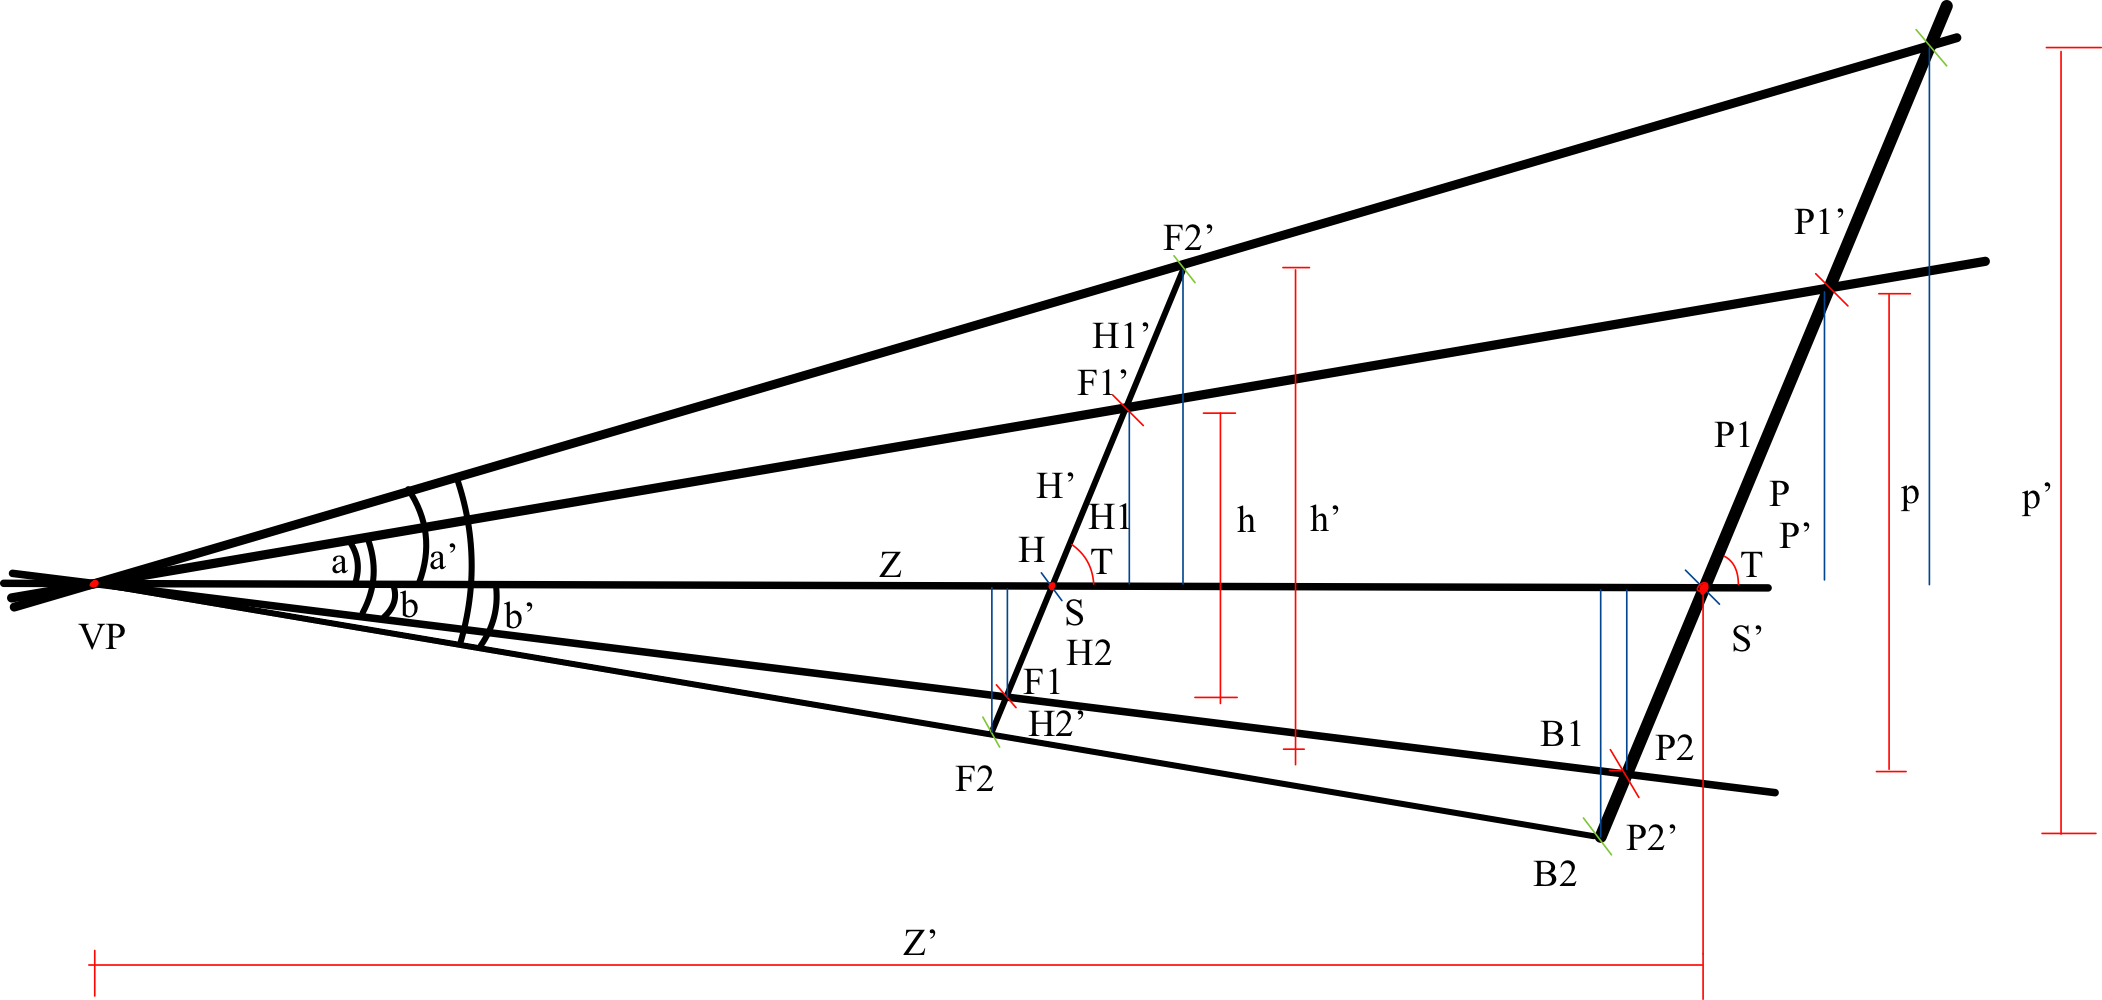
\includegraphics[width=1.0\textwidth]{Calculations2.jpeg}
    \caption{Generalized Projections from vanishing point}
    \label{fig: Generalized Projections from vanishing points}
\end{figure}
    
    \begin{Equation}[H]
        \begin{equation}
        \label{eq:equation1}
            \cot(a) = \frac{Z + H_1 \cos(T)}{H_1 \sin(T)}
        \end{equation}
        \caption{equation$8$}
    \end{Equation}
    
    \begin{Equation}[H]
        \begin{equation}
        \label{eq:equation1}
            \cot(a) = \frac{Z + P_1 \cos(T)}{P_1 \sin(T)}
        \end{equation}
        \caption{equation$9$}
    \end{Equation}
    
    \begin{Equation}[H]
        \begin{equation}
        \label{eq:equation1}
            \frac{Z}{H_1\sin(T)} + \cot(T) = \frac{Z'}{P_1\sin(T)} + \cot(T)
        \end{equation}
        \caption{equation$10$}
    \end{Equation}
    
    \begin{Equation}[H]
        \begin{equation}
        \label{eq:equation1}
            \frac{Z}{Z'} = \frac{H_1}{P_1} \quad \text{where } T \neq 0
        \end{equation}
        \caption{equation$11$}
    \end{Equation}
    
    \begin{Equation}[H]
        \begin{equation}
        \label{eq:equation1}
            \cot(b) = \frac{Z - H_2 \cos(T)}{H_2 \sin(T)}
        \end{equation}
        \caption{equation$12$}
    \end{Equation}
    
    \begin{Equation}[H]
        \begin{equation}
        \label{eq:equation1}
            \cot(b) = \frac{Z - P_2 \cos(T)}{P_2 \sin(T)}
        \end{equation}
        \caption{equation$13$}
    \end{Equation}
    
    \begin{Equation}[H]
        \begin{equation}
        \label{eq:equation1}
            \frac{Z}{H_2\sin(T)} - \cot(T) = \frac{Z'}{P_2\sin(T)} - \cot(T)
        \end{equation}
        \caption{equation$14$}
    \end{Equation}
    
    \begin{Equation}[H]
        \begin{equation}
        \label{eq:equation1}
            \frac{Z}{Z'} = \frac{H2}{P2} \quad \text{where } T \neq 0
        \end{equation}
        \caption{equation$15$}
    \end{Equation}
    
    \begin{Equation}[H]
        \begin{equation}
        \label{eq:equation1}
            \cot(a') = \frac{Z + H_1' \cos(T)}{H_1' \sin(T)}
        \end{equation}
        \caption{equation$16$}
    \end{Equation}
    
    \begin{Equation}[H]
        \begin{equation}
        \label{eq:equation1}
            \cot(a') = \frac{Z + P_1^{\prime} \cos(T)}{P_1^{\prime} \sin(T)}
        \end{equation}
        \caption{equation$17$}
    \end{Equation}
    
    \begin{Equation}[H]
        \begin{equation}
        \label{eq:equation1}
            \frac{Z}{H_1^{\prime}\sin(T)} + \cot(T) = \frac{Z^{\prime}}{P_1^{\prime}\sin(T)} + \cot(T)
        \end{equation}
        \caption{equation$18$}
    \end{Equation}
    
    \begin{Equation}[H]
        \begin{equation}
        \label{eq:equation1}
            \frac{Z}{Z'} = \frac{H_1^{'}}{P_1^{'}} \quad \text{where } T \neq 0
        \end{equation}
        \caption{equation$19$}
    \end{Equation}
    
    \begin{Equation}[H]
        \begin{equation}
        \label{eq:equation1}
            \frac{P_1}{H_1} = \frac{P_1^{'}}{H_1^{'}}
        \end{equation}
        \caption{equation$20$}
    \end{Equation}
    
    \begin{Equation}[H]
        \begin{equation}
        \label{eq:equation1}
            \cot(b') = \frac{Z - H_2^{\prime} \cos(T)}{H_2^{\prime}\sin(T)}
        \end{equation}
        \caption{equation$21$}
    \end{Equation}
    
    \begin{Equation}[H]
        \begin{equation}
        \label{eq:equation1}
            \cot(b') = \frac{Z - P_2^{\prime} \cos(T)}{P_2^{\prime}\sin(T)}
        \end{equation}
        \caption{equation$22$}
    \end{Equation}
    
    \begin{Equation}[H]
        \begin{equation}
        \label{eq:equation1}
            \frac{Z}{H_2^{\prime}\sin(T)} - \cot(T) = \frac{Z^{\prime}}{P_2^{\prime}\sin(T)} - \cot(T)
        \end{equation}
        \caption{equation$23$}
    \end{Equation}
    
    \begin{Equation}[H]
        \begin{equation}
        \label{eq:equation1}
            \frac{Z}{Z'} = \frac{H2^{'}}{P2^{'}} \quad \text{where } T \neq 0
        \end{equation}
        \caption{equation$24$}
    \end{Equation}
    
    \begin{Equation}[H]
        \begin{equation}
        \label{eq:equation1}
            \frac{P2}{H2} = \frac{P2^{\prime}}{H2^{\prime}}
        \end{equation}
        \caption{equation$25$}
    \end{Equation}
    
    \begin{Equation}[H]
        \begin{equation}
        \label{eq:equation1}
            \cot(a) + \cot(b) = \frac{Z + H1 \cos(T)}{H1 \sin(T)} + \frac{Z - H2 \cos(T)}{H2 \sin(T)}
        \end{equation}
        \caption{equation$26$}
    \end{Equation}

    \begin{Equation}[H]
        \begin{equation}
        \label{eq:equation1}
            \cot(a) + \cot(b) = \frac{Z}{\sin(T)} \quad \left(\frac{1}{H1} + \frac{1}{H2}\right) = \frac{Z^{\prime}}{\sin(T)} \quad \left(\frac{1}{P1} + \frac{1}{P2}\right)
        \end{equation}
        \caption{equation$27$}
    \end{Equation}
    
    \begin{Equation}[H]
        \begin{equation}
        \label{eq:equation1}
            \frac{Z}{Z'} = \frac{H_1 H_2 P}{P_1 P_2 H}
        \end{equation}
        \caption{equation$28$}
    \end{Equation}
    
    Similarly for cot(a')+cot(b')

    \begin{Equation}[H]
        \begin{equation}
        \label{eq:equation1}
            \frac{Z}{Z'} = \frac{(H_1^{\prime} H_2^{\prime}) P^{\prime}}{(P_1^{\prime} P_2^{\prime}) H^{\prime}}
        \end{equation}
        \caption{equation$29$}
    \end{Equation}
    
    Now, from eqn 7 and eqn 8,

    \begin{Equation}[H]
        \begin{equation}
        \label{eq:equation1}
            \frac{H}{P} = \frac{H^{\prime}}{P^{\prime}}
        \end{equation}
        \caption{equation$30$}
    \end{Equation}


From above, considering \ref{fig: Projections from vanishing point} and \ref{fig: Generalized Projections from vanishing points} as references for the calculations, we can see that when considering two objects of different sizes situated at the same place, at point S, if you extend the projection lines from a point, essentially creating projections for both objects at a particular distance, the ratio of the projection to the object, no matter the size of the object, is equal, given that the objects exist both above and below the point. Also, neither of the objects is in line with the projection line passing through point S.\newline

Some other observations can also be made. The ratio of the part of the object above point S to the part of the projection above the projection line through S is equal to the ratio of the object below point S to the part of the projection below the projection line through S. All these ratios—the size of the object to the size of the projection, the size of the parts of the object to the size of the parts of the projection—are also equal to the distance of the vanishing point to point S, and the distance of the vanishing point to the point where the projection line through S intersects the projection (S’).\newline

\begin{figure}[H]
    \centering
    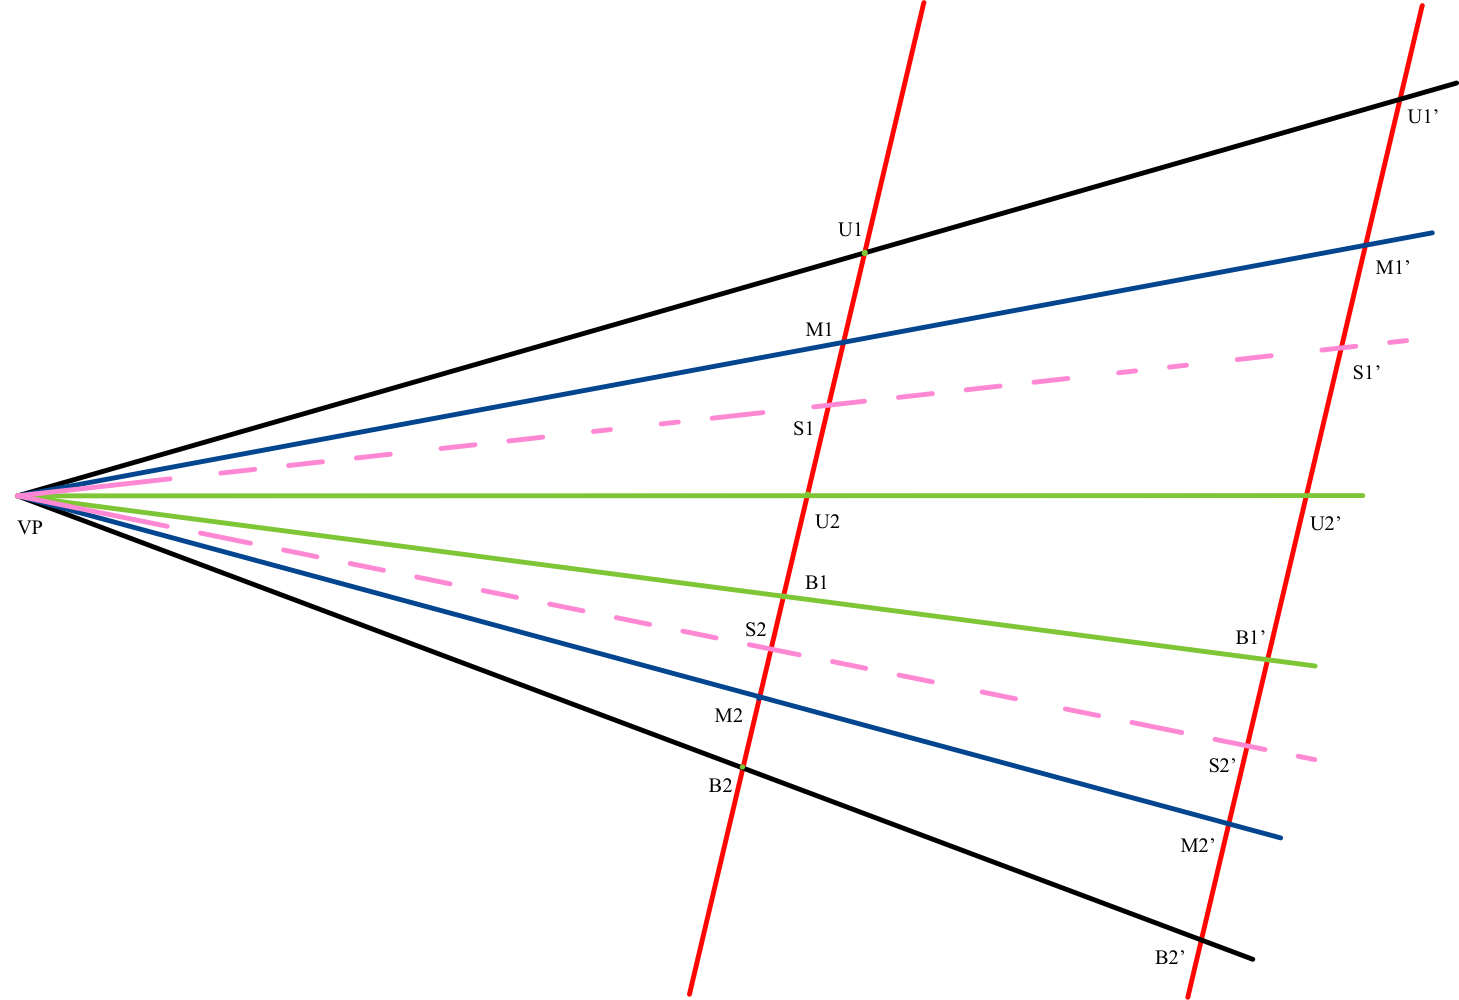
\includegraphics[width=1.0\textwidth]{Calculations3.jpeg}
    \caption{Objects of different heights at different altitudes}
    \label{fig: Objects of different heights at different altitudes}
\end{figure}

Now consider the following \ref{fig: Objects of different heights at different altitudes}\newline

We have three line segments U1U2=U, M1M2 =M, and B1B2 =B on the same line, and their projections U1'U2'=U', M1'M2' =M' and B1'B2 '=B' on the same line U1U2 and B1B2 do not overlap, whereas M1M2 has an overlap with both U1U2 and B1B2. That is also true for their projections using the observations from the previous sections. We can see that U'U=S1'S1=M'M, B'B=S2'S2=M'M, Hence, U'U=B'B=S1'S1=S2'S2.\newline

We can infer a few things from the above sections. The ratios of the line segments to the projections are equal, even though they do not intersect, as long as the line segments and their projections exist on the same lines, respectively. The ratio that we obtain is also independent of the length of the line segment as any change in the length of the line segment is also reflected in the projection. Now combining this information with the information that we have about the world in perspective view images, all parallel lines, depending on the number of vanishing points and the orientation of the parallel lines with respect to the vanishing point, either converge to a vanishing point in the image space or are parallel to each other in the image space. Either way, any object situated at a particular point, no matter its size or altitude from the ground plane, will be on the same line in the image space as in the real world. It will exist on the same Z coordinate, and that Z coordinate like all other Z coordinates will translate to a line passing through one of the vanishing points or a line parallel to all other Z coordinates.\newline

If we can standardize the positioning of the projection, we will obtain a standardized depth estimating system, which in combination with an absolute step size definition can be used to calculate and obtain the position/coordinates of the object/person.\newline

When a person is moving and remaining in contact with the ground plane—which typically is the case (i.e. walking or running)--and knowing when the person is not on the ground plane (i.e. jumping) would require a deep understanding of the environment and context clues since both having a deep understanding Of the environment and gathering context clues in a monocular image with no extra information is it a rather difficult and computationally expensive task and only covers a minor portion of the cases, we will assume that the person is always in contact with the ground plane.\newline

We consider the projection lines, passing through the bottom of the person/object and extend the line to reach the bottom line of the image. As shown above, we only need the distance of the bottom of the person/object from the projection point to the distance of the projection, the bottom line of the image from the projection point, measured along the projection line, we take the ratio of two and call it to be F Consider \ref{fig: Ratios on the ground plane}.\newline

\begin{figure}[H]
    \centering
    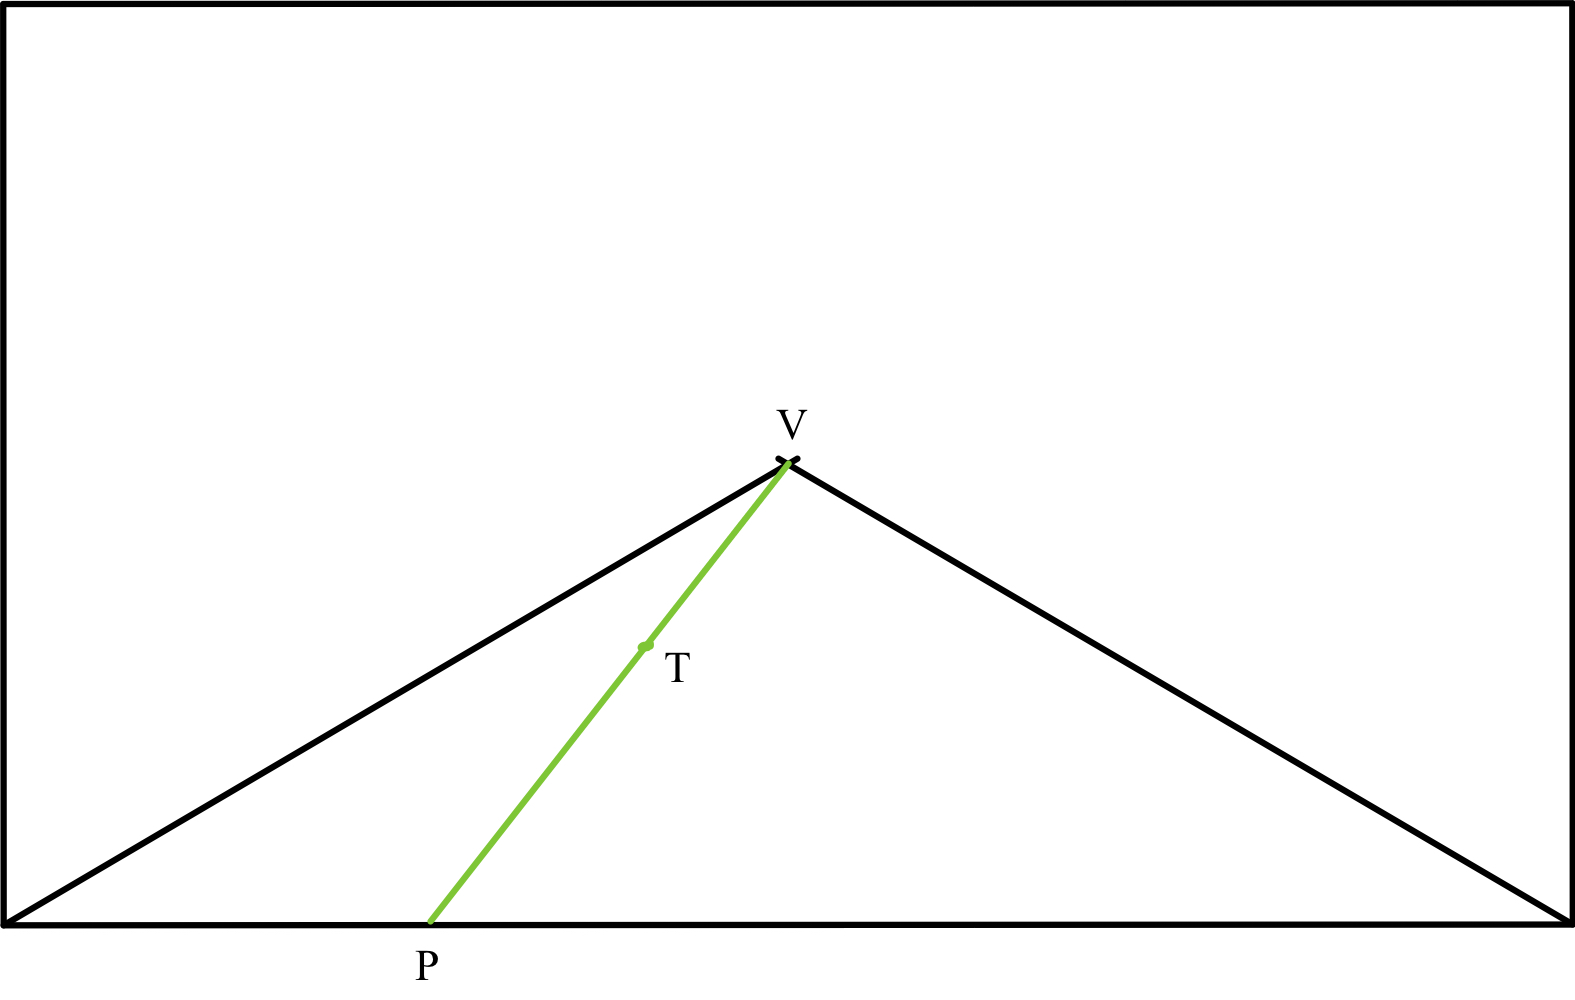
\includegraphics[width=1.0\textwidth]{Calculations4.jpeg}
    \caption{Ratios on the ground plane}
    \label{fig: Ratios on the ground plane}
\end{figure}

    \begin{Equation}[H]
        \begin{equation}
        \label{eq:equation1}
            VT = S
        \end{equation}
        \caption{equation$31$}
    \end{Equation}
    
    \begin{Equation}[H]
        \begin{equation}
        \label{eq:equation1}
            VP = S'
        \end{equation}
        \caption{equation$32$}
    \end{Equation}
    
    \begin{Equation}[H]
        \begin{equation}
        \label{eq:equation1}
            F = \frac{S}{S'} = \frac{VT}{VP}
        \end{equation}
        \caption{equation$33$}
    \end{Equation}


We further need a standardized point to extend the projection lines from. There are a few options that we can consider. The first would be to use the vanishing points, but depending upon the view angle and the positioning of the room, there can be multiple vanishing points. Choosing different points would give different coordinates for people/objects. The second option to tackle would be to consider a point that accounts for all the vanishing points. In the case of one vanishing point perspective view, that would be the vanishing point itself. In the case of two vanishing point perspective view, it would be the center of the line joining both of the vanishing points. And in the case of the three vanishing point perspective view, it would be the centroid of the triangle formed by the three vanishing points. The third option would be to consider the center of the image frame. This works on the same idea as the other two cases, requires the least calculations, and is the easiest to implement; however, it is prone to errors.\newline

If the center of the image is chosen to be the projection point, and the positioning of the camera and the room are at an extreme position/angle to each other. There can be cases where the ground plane crosses the center of the image frame, which will lead to some errors because at that point there can be a person/object that is placed directly at the projection point and our calculations for that person/object will indicate that they are standing at infinity, which would be wrong. Such a scenario can be avoided by using the second option, which encapsulates the idea of using all of the vanishing points and will always yield the correct results. However, for the purpose of testing, we will be using the third option, as it conveys the same idea and the conditions that lead to errors are rare.\newline

The next step in the problem is to define an absolute origin. For our coordinate system, we again have a few options to consider. We could use the point we are using to extend the projection lines from (i.e. the projection point) as the origin, but since it is supposed to be a representation of the vanishing points, it is infinitely far from our plane and will place all the objects in consideration at infinity. The second option is to place the origin at one of the corners of the room. At first, this feels intuitive and would make translating the coordinates to the real world easy, which helps open more practical use cases. However, calculating the coordinates of the person/object, with respect to a separate point as compared to one not directly related to the point being used to calculate the depth of the person requires additional calculations at each step. The third option—to place the origin—would be to consider a point that relates to one being used to extend the projection lines from, and one that is close enough to the image plane. Hence, we can project the point directly to the bottom of the image and consider the point at the ground plane that the projection corresponds to, to be our origin. We can then calculate the position of all the people/objects in consideration with respect to this, the coordinates of the corners, and the walls can also be calculated using the same logic. After calculation, if needed, the original can be shifted to any one of these corners of the room by simply translating the coordinate system.\newline

Now that we have the original place, the next step is to turn the ratio that we have corresponding to the depth into absolute Z coordinates. To do so we still need to define a step size in terms of the image space this can be defined either in terms of an absolute number of pixels add the image plane, or as a factor of the dimensions of the image which can then be translated to a number of pixels. \ref{fig:Step Size} Shows the step size at the image plane, \ref{fig: Step Size label} focuses on the bottol left half of the room in \ref{fig:Step Size} and provides labels for the step size and the projection point.\newline

\begin{figure}[H]
    \centering
    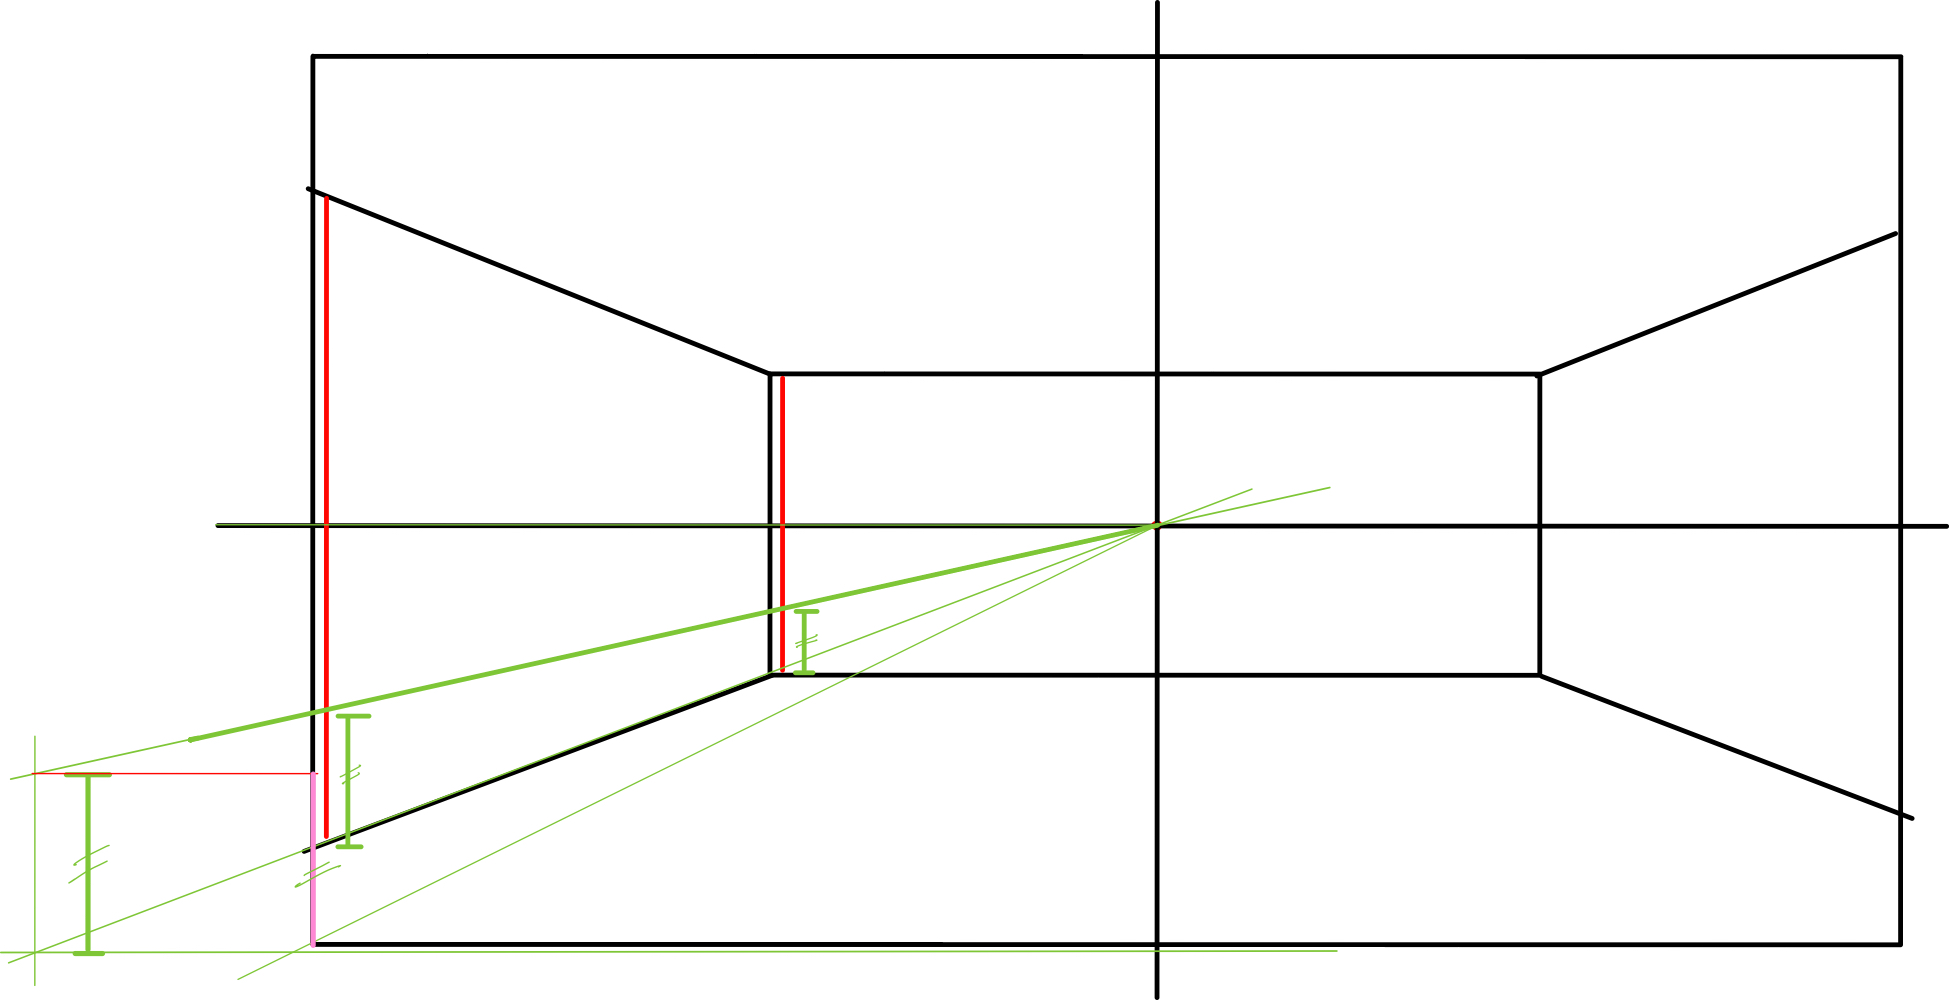
\includegraphics[width=1.0\textwidth]{Calculations5.jpeg}
    \caption{Step Size}
    \label{fig:Step Size}
\end{figure}

\begin{figure}[H]
    \centering
    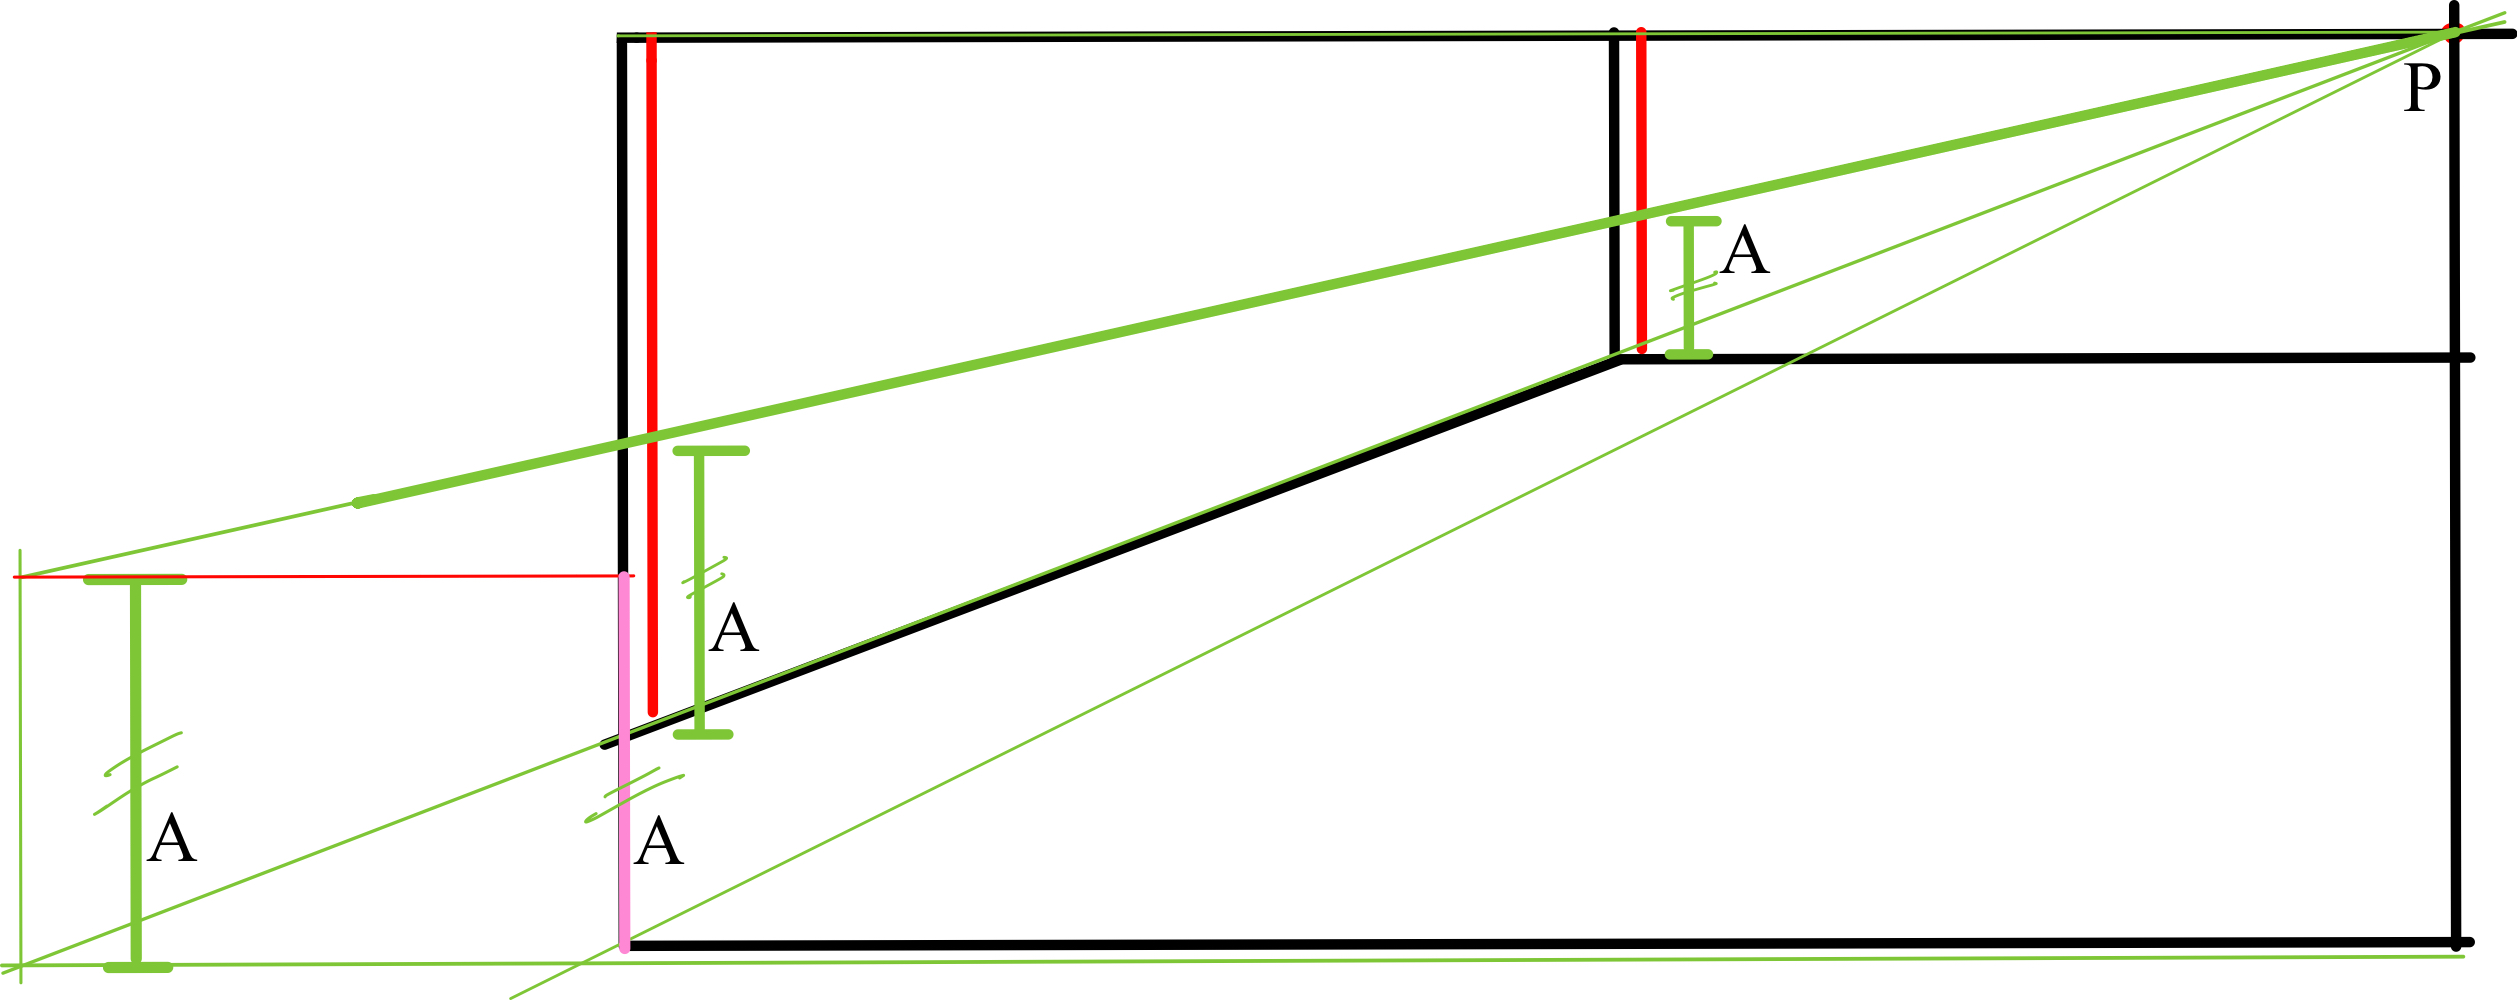
\includegraphics[width=1.0\textwidth]{Calculations6.jpeg}
    \caption{Step Size labels}
    \label{fig: Step Size label}
\end{figure}

Considering the image we can assume the step size at the image plane to be a and the distance from the projection point to the base of the image plan projected on the image to BS as the projection point is at infinity, there needs to be infinite steps, each of step size a taken to reach it, all the steps are represented in S and are gradually getting smaller and smaller. This can be represented as an infinitely decreasing geometric progression whose first term is a and the sum is S using these two values we can calculate the common ratio of the geometric progression.\newline

\begin{Equation}[H]
        \begin{equation}
        \label{eq:equation1}
            S = \frac{A}{1 - r}
        \end{equation}
        \caption{equation$34$}
    \end{Equation}
    
    \begin{Equation}[H]
        \begin{equation}
        \label{eq:equation1}
            1 - r = \frac{A}{S}
        \end{equation}
        \caption{equation$35$}
    \end{Equation}
    
    \begin{Equation}[H]
        \begin{equation}
        \label{eq:equation1}
            r = 1 - \left(\frac{A}{S'}\right) \quad \text{where } S > A
        \end{equation}
        \caption{equation$36$}
    \end{Equation}


By convention, we will consider the distance between the projection point, and the bottom corner of the image which is further from the projection point.\newline

\begin{figure}[H]
    \centering
    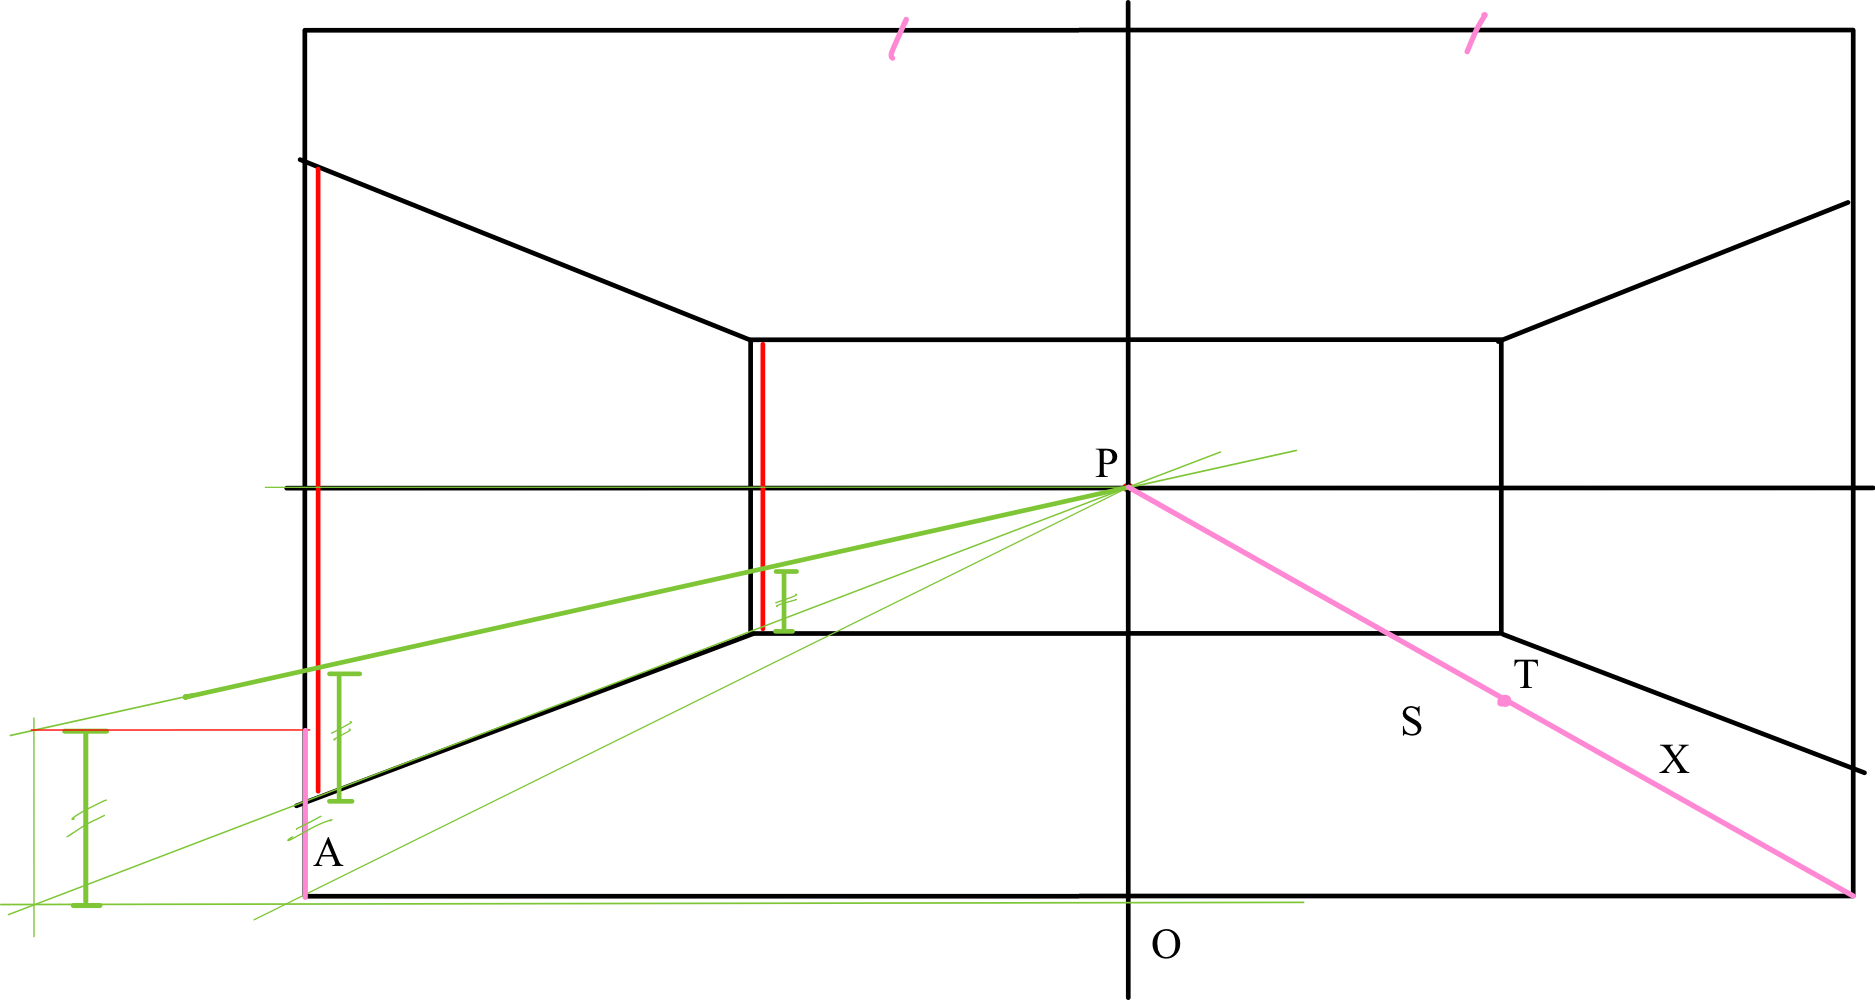
\includegraphics[width=1.0\textwidth]{Calculations7.jpeg}
    \caption{Support for depth calculation}
    \label{fig: Support for depth calculation}
\end{figure}

\begin{figure}[H]
    \centering
    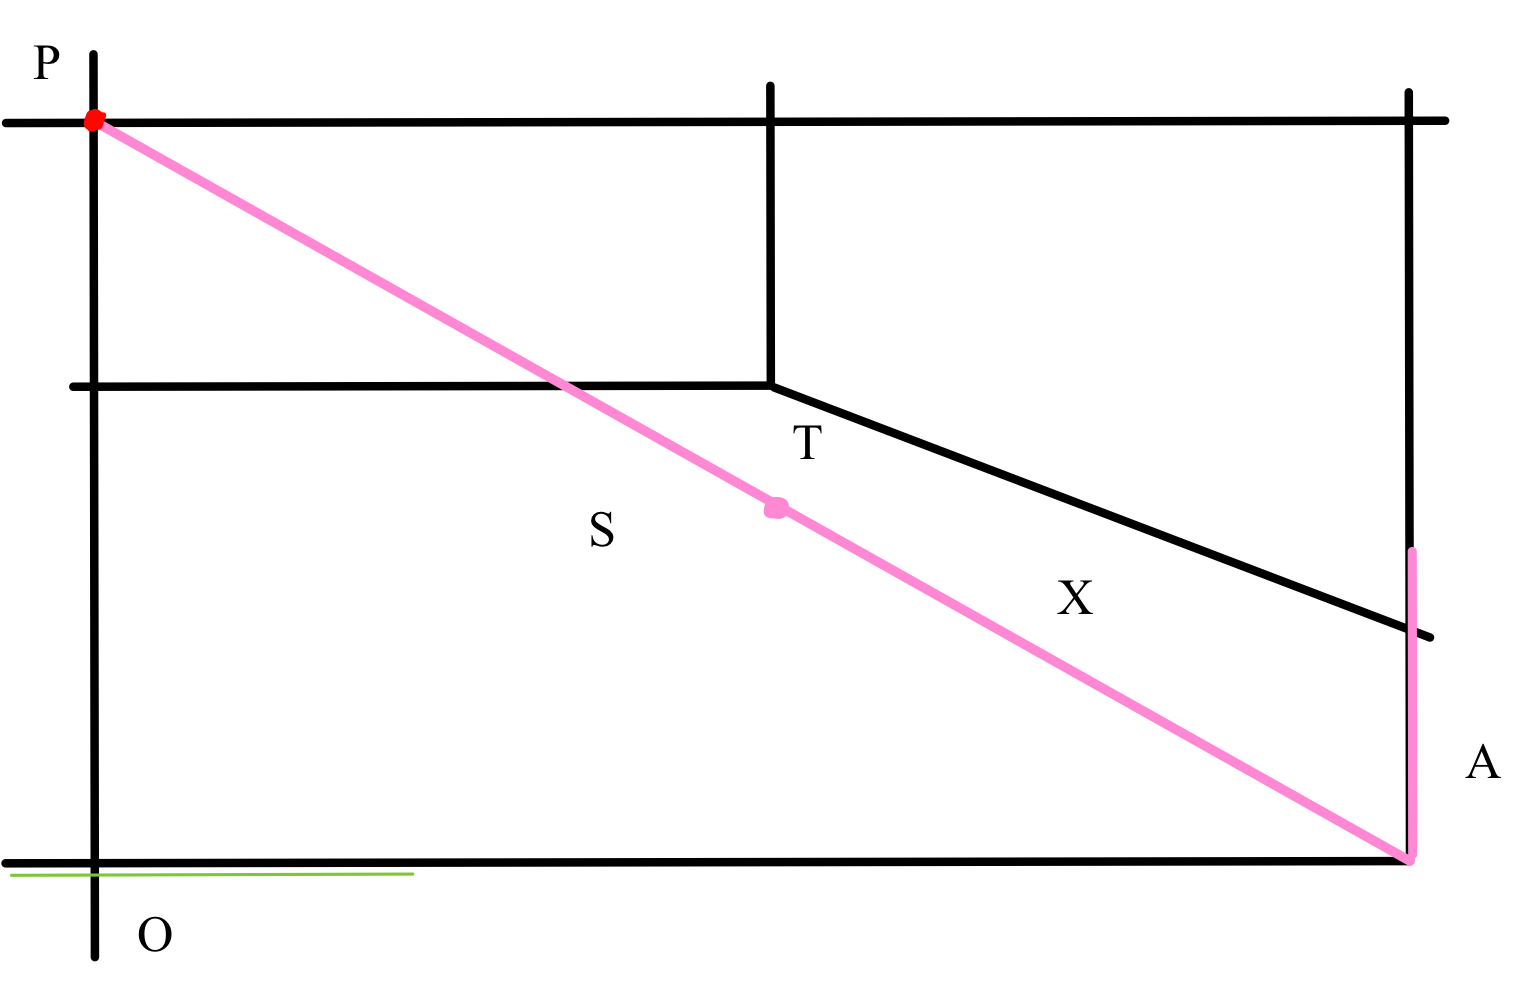
\includegraphics[width=1.0\textwidth]{Calculations8.jpeg}
    \caption{Support for depth calculation}
    \label{fig: Support for depth calculation labels}
\end{figure}

\ref{fig: Support for depth calculation} shows a room with projection line extend form the projection point, and \ref{fig: Support for depth calculation labels} focuses on the bottom right quarter of the image and provides labels to support the following calculations.\newline

Now, for a person at a certain depth with the projection at the image plane as X, we take n steps to reach the depth, as X is the sum of N steps that are part of a metric progression we can calculate n as follows.\newline


\begin{Equation}[H]
        \begin{equation}
        \label{eq:equation1}
            X = \frac{A(1 - r^n)}{1 - r}
        \end{equation}
        \caption{equation$37$}
    \end{Equation}
    
    \begin{Equation}[H]
        \begin{equation}
        \label{eq:equation1}
            \frac{X(1 - r)}{A} = 1 - r^n
        \end{equation}
        \caption{equation$38$}
    \end{Equation}
    
    \begin{Equation}[H]
        \begin{equation}
        \label{eq:equation1}
            r^n = 1 - \frac{X(1 - r)}{A}
        \end{equation}
        \caption{equation$39$}
    \end{Equation}
    
    \begin{Equation}[H]
        \begin{equation}
        \label{eq:equation1}
            r^n = 1 - \frac{X}{S} \quad \text{where } S = \frac{A}{1 - r}
        \end{equation}
        \caption{equation$40$}
    \end{Equation}
    
    \begin{Equation}[H]
        \begin{equation}
        \label{eq:equation1}
             n \log(r) = \log\left(1 - \frac{X}{S}\right)
        \end{equation}
        \caption{equation$41$}
    \end{Equation}
    
    \begin{Equation}[H]
        \begin{equation}
        \label{eq:equation1}
            n = \frac{\log\left(1 - \frac{X}{S}\right)}{\log(r)}
        \end{equation}
        \caption{equation$42$}
    \end{Equation}
    
    \begin{Equation}[H]
        \begin{equation}
        \label{eq:equation1}
            n = \log_r(F)
        \end{equation}
        \caption{equation$43$}
    \end{Equation}
    
    \begin{Equation}[H]
        \begin{equation}
        \label{eq:equation1}
            F = 1 - \frac{X}{S}
        \end{equation}
        \caption{equation$44$}
    \end{Equation}


Here F is nothing but the ratio of the distance of the person/object from the projection point to the distance of the projection of the site person/object from the projection point calculated in the space calculation of F was also discussed in the previous sections.\newline

\begin{figure}[H]
    \centering
    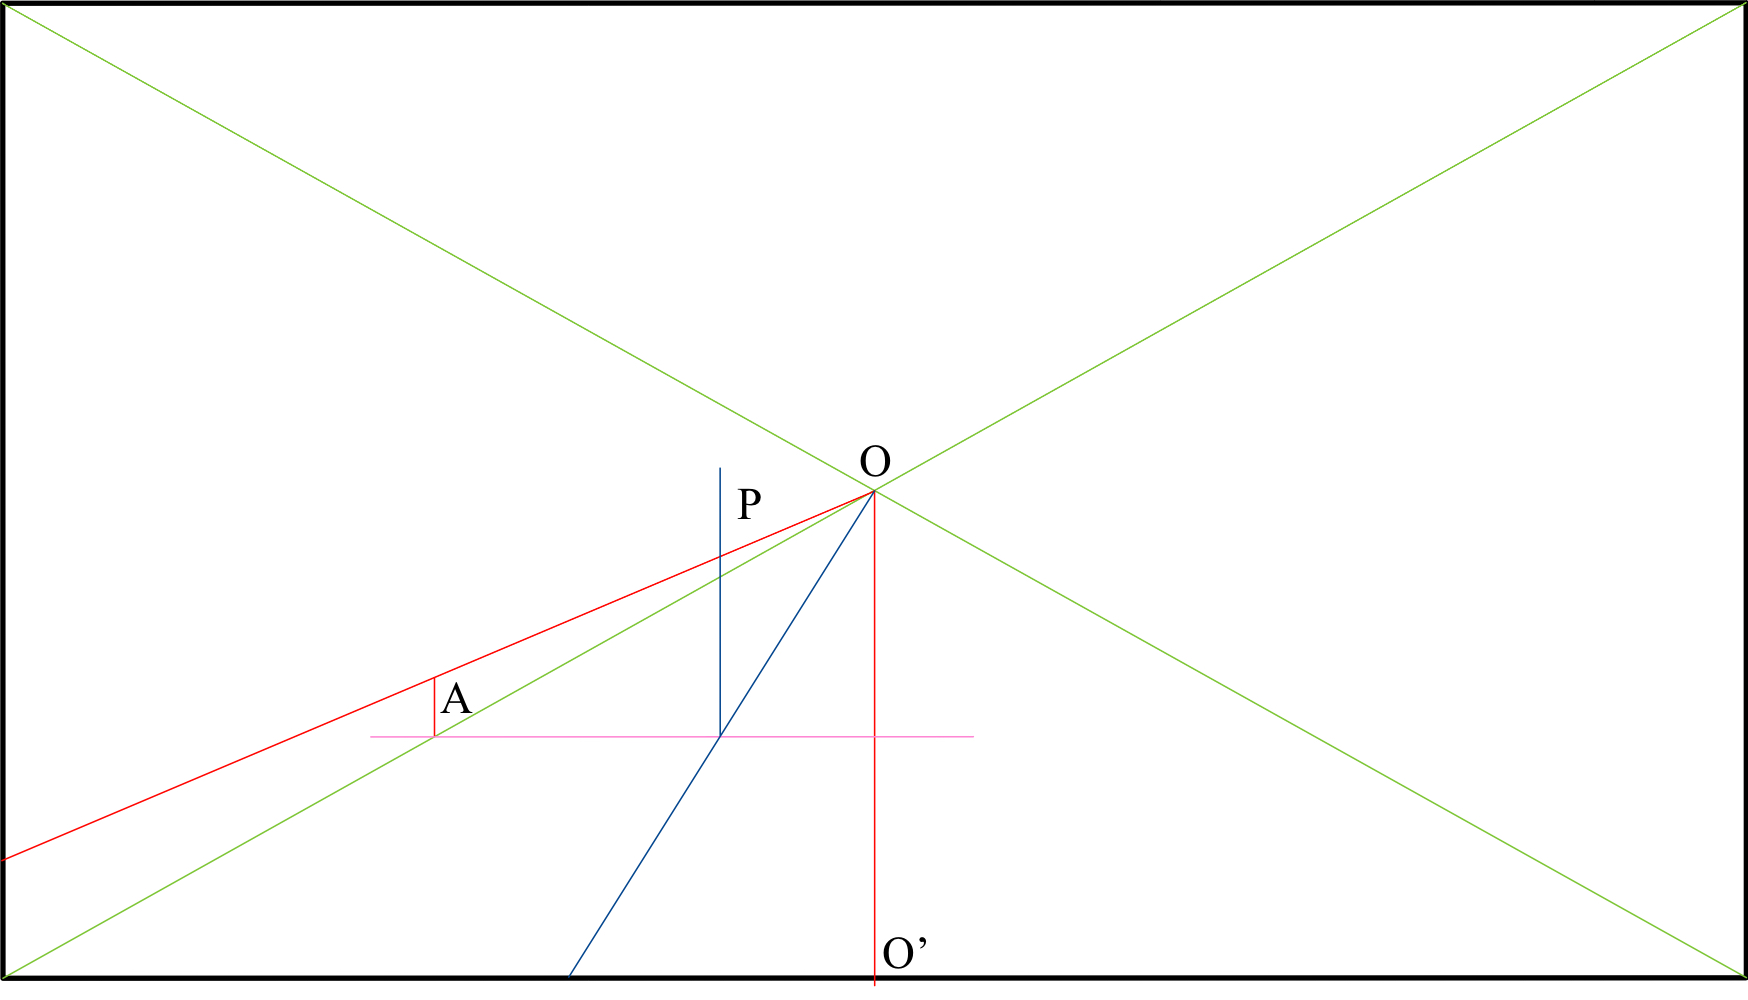
\includegraphics[width=1.0\textwidth]{Calculations9.jpeg}
    \caption{Coordinate System}
    \label{fig: Coordinate System}
\end{figure}

\ref{fig: Coordinate System} Shows the Projection point O, the origin O’, and a person represented by the lime P. In the figure, the line connecting the origin to the projection point OO' is given by x= y=0.\newline

The following Figures, \ref{fig: Medium sized object}, \ref{fig: Tall person}, and \ref{fig: Extremely small object}, show one of the more extreme angle placements of the camera relative to the scene. All images have been clicked from the same camera angle and show subjects of different heights standing at the same position in the real world. P represents the projection point and is also the centroid of the three vanishing points, the point on the ground plane where the subject stands is represented by Z and the point of intersection of the projection line with the image edge is Z’. Since the camera is not moving P is the same and because the subjects all stand at the same point Z for all three is also the same, hence the the ratio PZ/PZ’ is the same in all three cases resulting in the same coordinates.\newline

\begin{figure}[H]
    \centering
    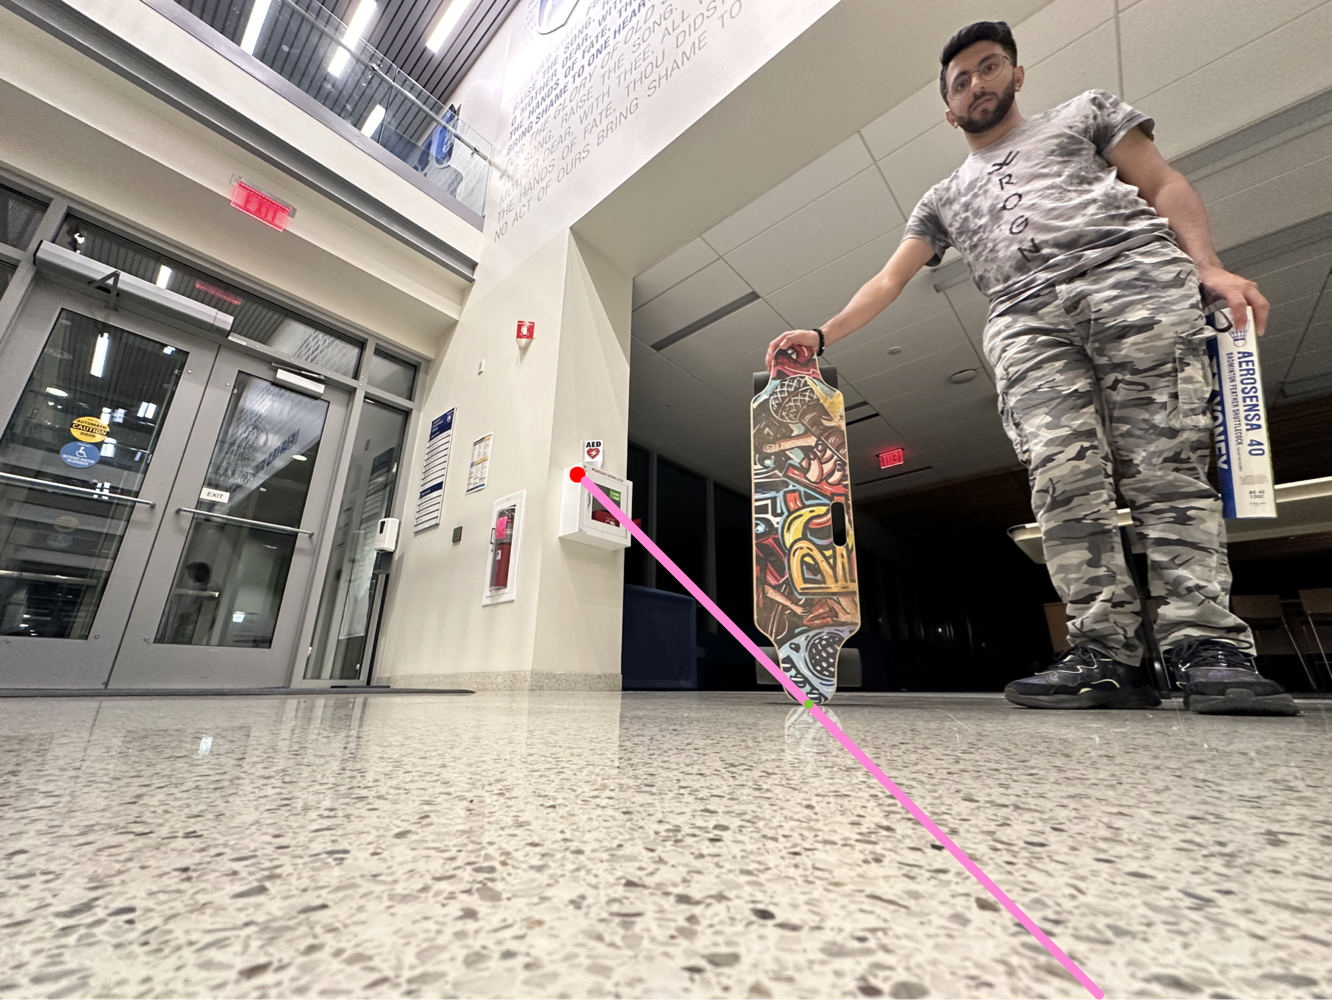
\includegraphics[width=0.9\textwidth]{3vpmo.jpeg}
    \caption{Medium sized object}
    \label{fig: Medium sized object}
\end{figure}

\begin{figure}[H]
    \centering
    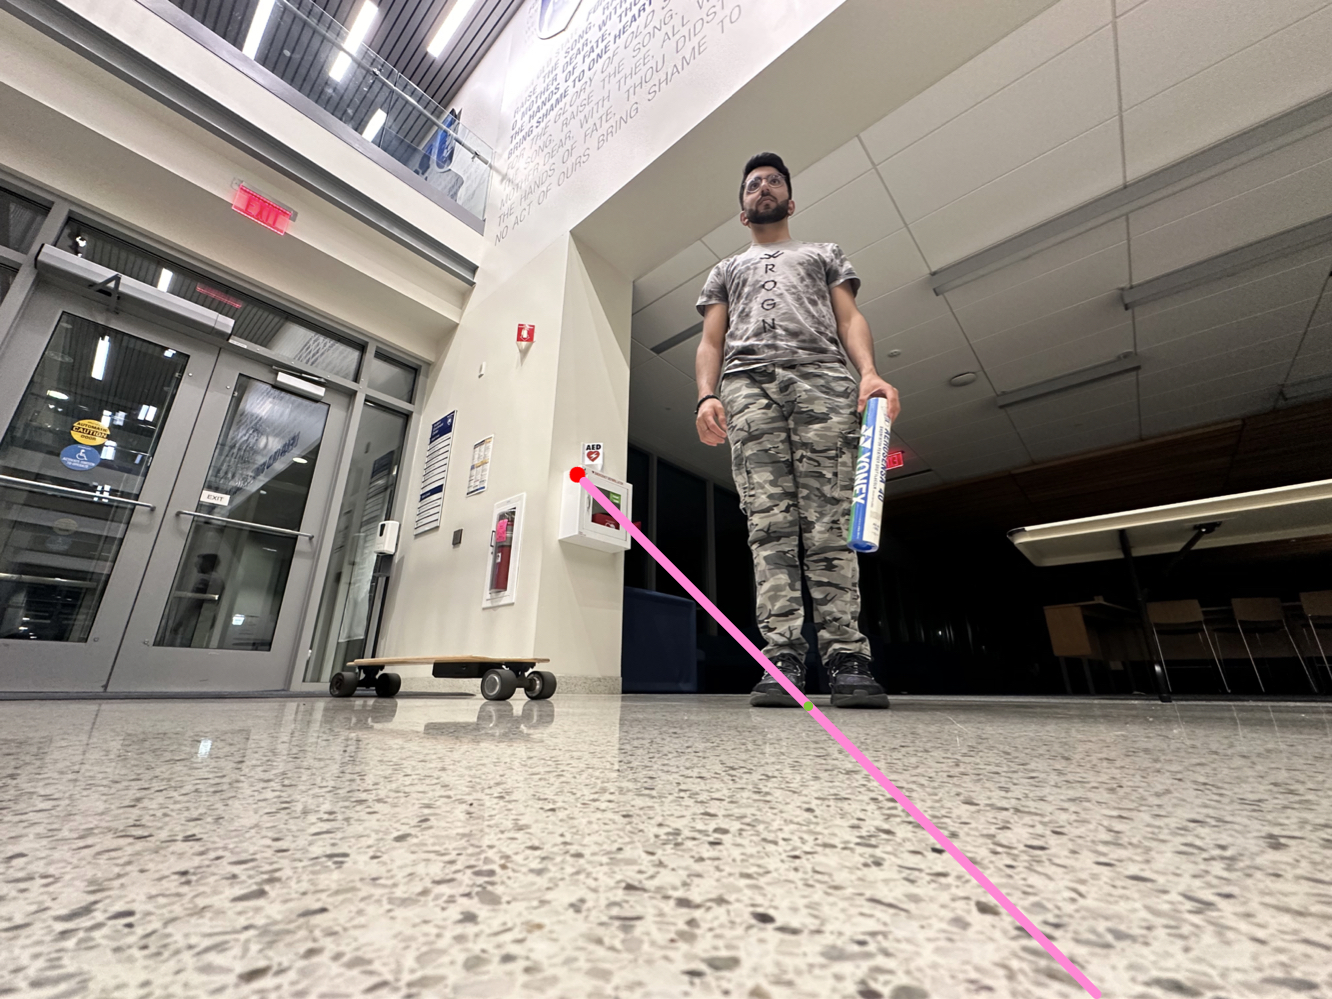
\includegraphics[width=0.8\textwidth]{3vpto.jpeg}
    \caption{Tall person}
    \label{fig: Tall person}
\end{figure}

\begin{figure}[H]
    \centering
    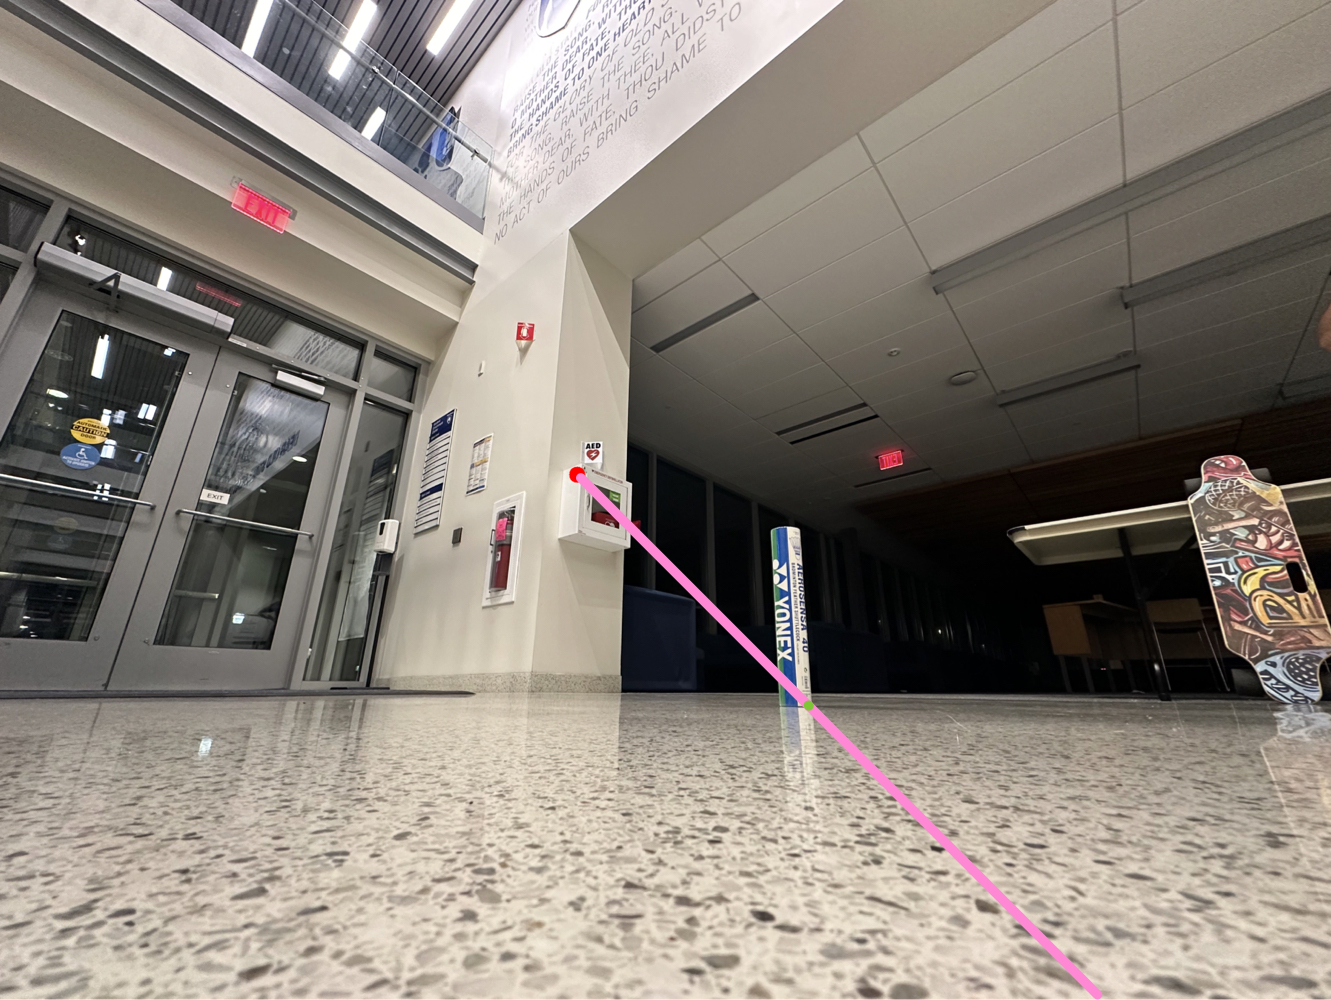
\includegraphics[width=0.8\textwidth]{3vpso.jpeg}
    \caption{Extremely small object}
    \label{fig: Extremely small object}
\end{figure}

\section{Tracking}

After the coordinates of any person/object have been calculated in one frame, we only need to continuously detect them in consecutive frames. The accuracy and the precision of the detection depend on the model being used to detect the person/object for testing. we are using Yolo as it provides a high accuracy whilst being light enough to be run on most devices locally. However, looking at the entire image space in each frame can be computationally expensive. Therefore, we will implement some techniques to reduce the computation cost and make the overall algorithm faster.\newline

The aim is to mimic the way that living organisms track objects moving through their field of view. The idea is to create a small dynamic window around the object/person once they are detected and then use predictive programming to predict where the person might be in the next frame And move the window to the predicted place of the image space. We keep buffer space around the person and use the coordinates of the subject within the image space from the past few frames to calculate the average speed and the direction of motion of the person/object to estimate their position in the next frame. we also create a feedback globe as each time the set of past frames being used to calculate the position is updated. The size of the buffer can also be changed, depending upon the speed of the person/object, and the window can be skewed in the direction of the motion.\newline
